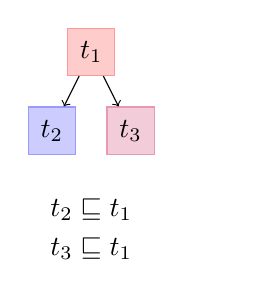
\begin{tikzpicture}
[   cnode/.style={draw=black,fill=#1,minimum width=3mm,circle},
    rnode/.style={draw=#1!40,fill=#1!20,minimum width=6mm, minimum height=6mm, rectangle},
    gnode/.style={draw=gray!40,fill=gray!20,circle,scale=0.5},
    gline/.style={gray!40}
]




\node[rnode=red] (a) at (5.8, 1.5) {$t_1$};
\node[rnode=blue] (b) at (5.3, 0.5) {$t_2$};
\node[rnode=purple] (c) at (6.3, 0.5) {$t_3$};

\node at (5.8, -0.5) {$t_2 \sqsubseteq t_1$};
\node at (5.8, -1) {$t_3 \sqsubseteq t_1$};
\draw[->] (a) -- (b) {};
\draw[->] (a) -- (c) {};
\node at (7.5, 0) {};
\end{tikzpicture}